\documentclass[11pt, oneside]{article}
\usepackage[margin=0.75in]{geometry}
\geometry{letterpaper}
\usepackage{graphicx}
\usepackage{amssymb}
\usepackage{amsmath}
\usepackage{enumitem}
\usepackage{mathtools}
\usepackage{xcolor}
\usepackage{framed}
\usepackage{listings}
\usepackage{xparse}

%\graphicspath{{C:\\Users\\HP  user\\Documents\\GitHub\\Project-Euler\\LaTeX writeups\\Problem 246\\}}

% block comment. Usage "\comment{ comment goes here }"
\newcommand{\comment}[1]{}

% ======== shorthands ========= %
\newcommand{\ccontra}{\ensuremath{\Rightarrow&\Leftarrow}}	% => & <= (centered contradiction)
\newcommand{\contra}{\ensuremath{\Rightarrow\Leftarrow}}	% => <= (contradiciton)
\newcommand{\inv}[1]{\ensuremath{#1^{-1}}}              	% multiplicitive inverse
\newcommand{\nin}{\ensuremath{\notin}}                  	% \notin
% shorthand for common math sets
\newcommand{\NN}{\ensuremath{\mathbb N}}
\newcommand{\nn}{\ensuremath{\mathbb N}}
\newcommand{\ZZ}{\ensuremath{\mathbb Z}}
\newcommand{\zz}{\ensuremath{\mathbb Z}}
\newcommand{\QQ}{\ensuremath{\mathbb Q}}
\newcommand{\qq}{\ensuremath{\mathbb Q}}
\newcommand{\RR}{\ensuremath{\mathbb R}}
\newcommand{\rr}{\ensuremath{\mathbb R}}
\newcommand{\CC}{\ensuremath{\mathbb C}}
\newcommand{\cc}{\ensuremath{\mathbb C}}
\newcommand{\FF}{\ensuremath{\mathbb F}}
\newcommand{\ff}{\ensuremath{\mathbb F}}
% ======== shorthands ========= %

% ==== formatting for code ==== %
%\usepackage{listings}
%\usepackage{xcolor}
\definecolor{codegreen}{rgb}{0,0.6,0}
\definecolor{codegray}{rgb}{0.5,0.5,0.5}
\definecolor{codepurple}{rgb}{0.58,0,0.82}
\definecolor{backcolor}{rgb}{0.95,0.95,0.92}
% in-line code command
\newcommand{\code}[1]{\colorbox{backcolor}{\texttt{#1}}}
\lstdefinestyle{mystyle}{
    backgroundcolor=\color{backcolor},   
    commentstyle=\color{codegreen},
    keywordstyle=\color{magenta},
    numberstyle=\tiny\color{codegray},
    stringstyle=\color{codepurple},
    basicstyle=\ttfamily\footnotesize,
    breakatwhitespace=false,         
    breaklines=true,                 
    captionpos=b,                    
    keepspaces=true,                 
    numbers=left,                    
    numbersep=5pt,                  
    showspaces=false,                
    showstringspaces=false,
    showtabs=false,                  
    tabsize=4
}
\lstset{style=mystyle}
% ===== example of usage ====== %
% \begin{lstlisting}[language=Python caption=Python Example]
% 	for x in range(5):
%		print(x)
% \end{lstlisting}
% ==== formatting for code ==== %

\title{Tangents to an Ellipse}
\author{John Butler}
\date{}


\begin{document}
\maketitle

\begin{enumerate}
	% TODO maybe try to restate problem?
	\item \textbf{Finding an equation for the ellipse}\\
		The way it's described in the problem, the ellipse isn't very usable. I had a hard time thinking about the ellipse in the way it was given.
		Normally, I would like to work with ellipses in the form $\left(\frac {x - x_0} a\right)^2 + \left(\frac {y-y_0} b\right)^2 = 1$. If we could 
		figure it out in terms of $M$, $G$, and $r$, that would be wonderful.
		
		Maybe it's clear from the first animation on PE if you're familiar with ellipses, but $M$ and $G$ are the foci of $e$. A property the foci have is
		that for every point $E$ on the ellipse, the distance between $E$ and the two foci are constant. In the problem descripion, we are told that 
		$\overline{EG}=\overline{EU}$ and if we extend $\overline{EU}$ we hit $M$. Because $c$ is a circle, we know that $\overline{MU}$ is constant.
		so $\overline{EM} + \overline{EU}$ is constant, and since $\overline{EU}=\overline{EG}$, $\overline{EM} + \overline{EG}$ is constant. Furthermore,
		$\overline{EM}+\overline{EG}=r$. We can then gather that $M$ and $G$ are the foci of this ellipse.

		Now that we know that $M$ and $G$ are the foci, if we shift them so that they are opposite each other, the ellipse will be centered and I won't
		have to worry about the shifting terms $x_0$ or $y_0$ in the equation. The new $M$ and $G$ are being shifted by $-3000$ in the $x$ direction and
		$-1500$ in the $y$ direction to land us at $M=(-5000,0)$ and $G=(5000,0)$.

		Now let's find $a$ and $b$, the semi-major and semi-minor axes. It's easiest to find $a$ first in my opinion. Let's think about the right-most 
		point of the ellipse and call it $E$. We know that $\overline{EG}=\overline{EU}$. We also know $\overline{EU}$ can be extended to $M$, the center 
		of the circle $c$. Because an ellipse is symmetric, we know that the distance between $M$ and the left edge is the same as 
		$\overline{EG} = \overline{EU}$, the whole width of the ellipse is the same as the radius, so $2a=r$ and $a = \frac 1 2 r = 7500$.

		$b$ is a little trickier, but we start off the same. Consider the topmost point, say $E$. We know that $\overline{EM}=\overline{EG}$ because
		%TODO add pictures
		ellipses are symmetric. We can now bisect $MEG$ and get two right traingles. Comparing with lengths we already figured out, 
		\begin{align*}
			\left(\frac{\overline{MG}} 2\right)^2 + b^2 &= \left(\frac r 2\right)^2\\
			b &= \frac12\sqrt{r^2 - \overline{MG}^2}\\
			&\approx 5590.17
		\end{align*}
		
		So now we have our equation!

		$$\left(\frac x a\right)^2 + \left(\frac y b\right)^2 = 1$$

		For ease of further manipulating, I'm not going to replace $a$ and $b$ with their values.
		
		\newpage
	\item \textbf{Small reframing of the problem.}\\
		It seems obvious, at least to me, that all of the points we want to consider are ``connected.'' That is there's some (probably convex) shape that 
		all of the points we're trying to find are located inside. My intuition told me that this was an ellipse but I was wrong. I went through the 
		trouble of mapping out the points and here's what it looks like:

		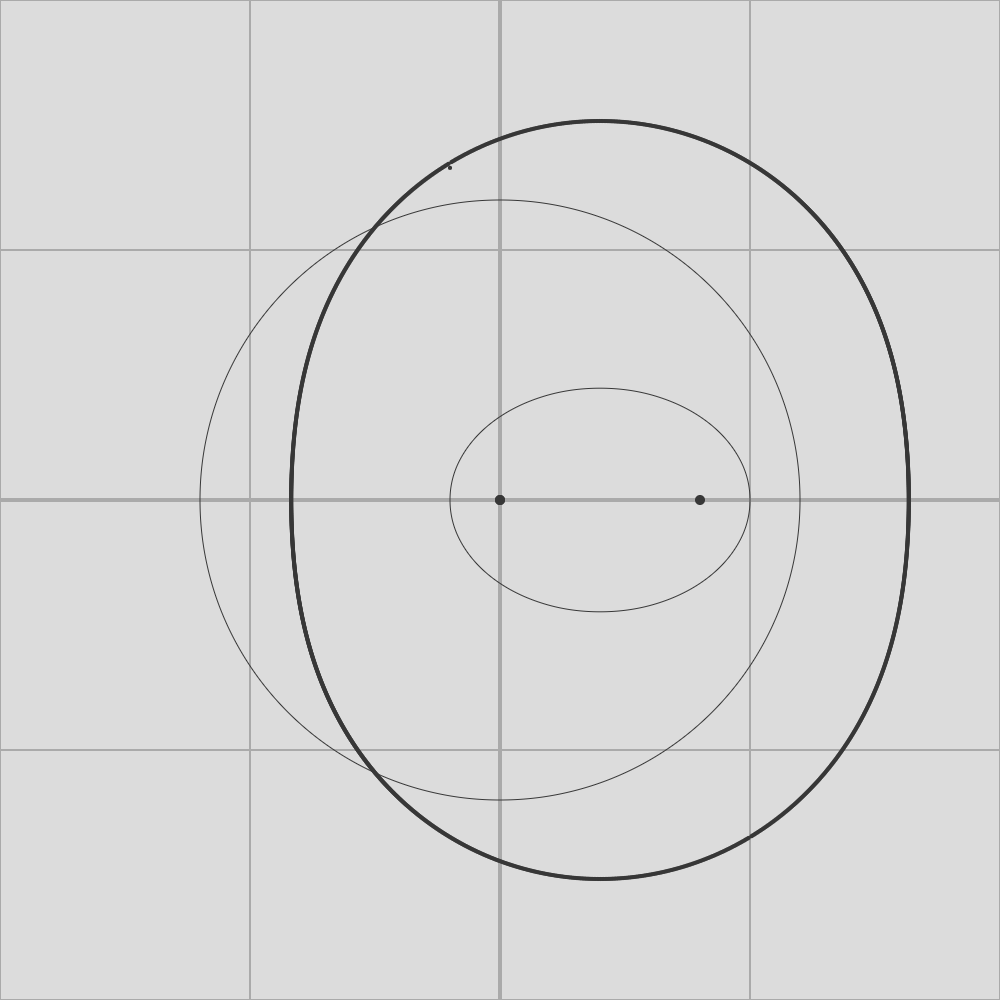
\includegraphics[height=5cm]{boundary to search}
		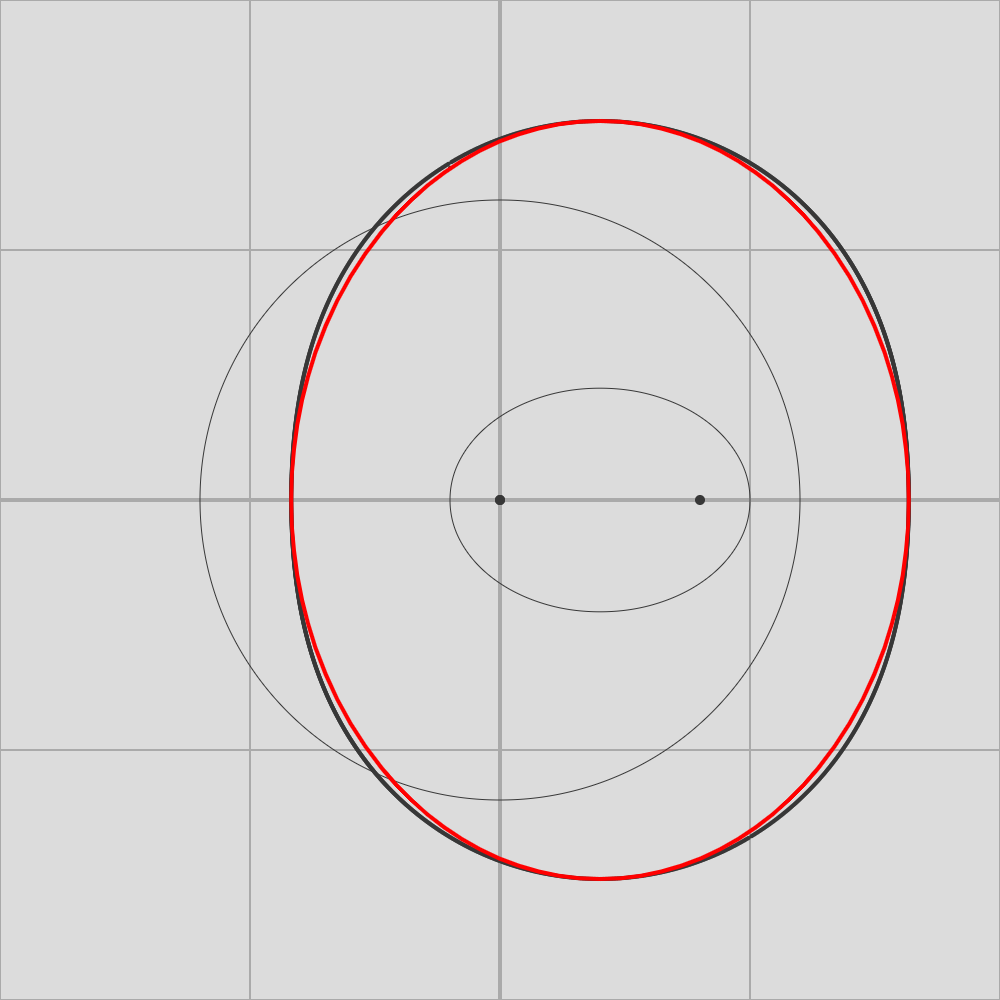
\includegraphics[height=5cm]{boundary is not ellipse} 
		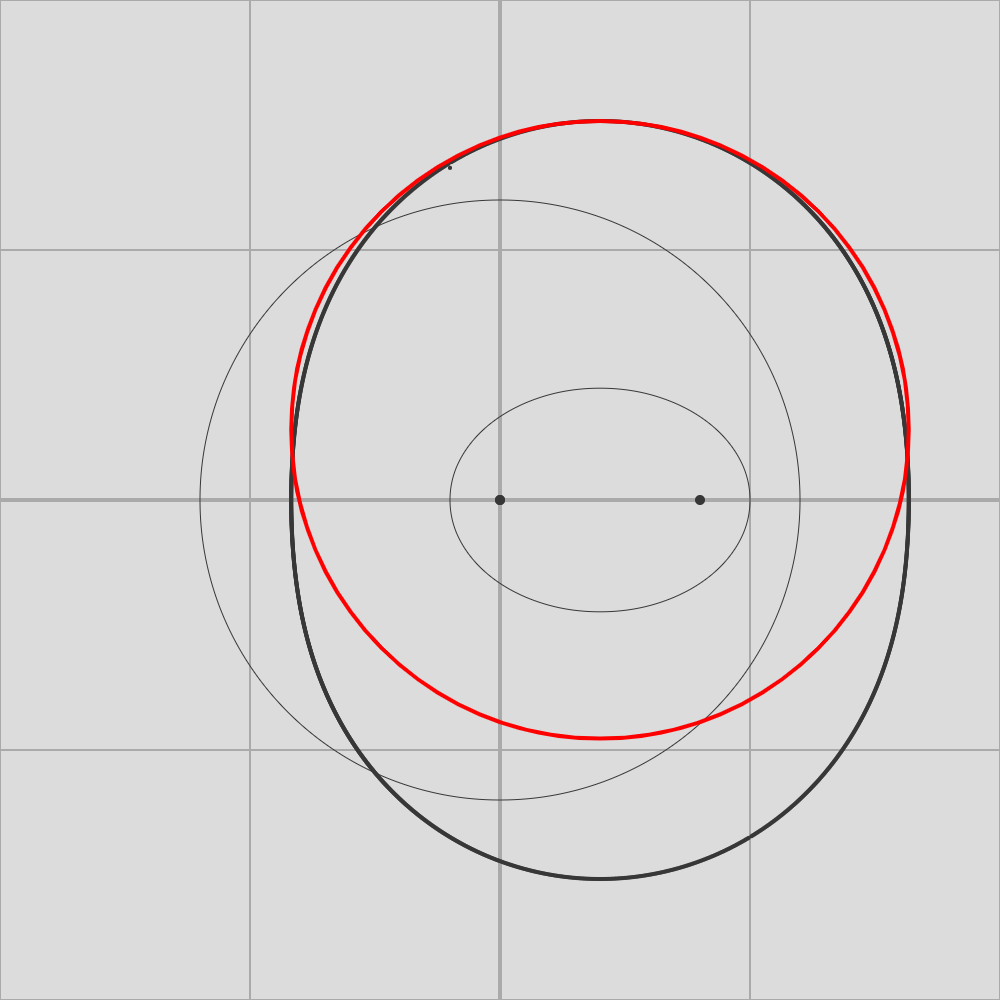
\includegraphics[height=5cm]{boundary not circle}

		I've overlaid an ellipse and a circle to show that it's not either of those. I thought it looked a little like two semi circles joined by a line, 
		so I wanted to see what that looked like. Still I could not find a satisfying formula for the perimeter of the ellipse. I have found an ugly one
		that you will see later on. It involved $\arctan$, so I suspect that it's not able to be written cleanly.

		It's very much like we're trying to solve for the area of this weird shape, so that's why I was so determined to find an equation. 
		I'm not sure if we could land on the exact solution, but I thought maybe it would be possible to integrate to find the area.

	\item \textbf{Finding the points of tangency}\\
		At a high level, the solution I came up with involves finding the nearest lattice point to the edge for each y value to calculate how many there
		are in total on that row. But to do that, I need to be able to find the tangents and then their angle.

		To start, let's find the derivative of the ellipse. Since we're finding tangents, we're gonna need to know the slope for any given point on the
		ellipse. I will use implicit differentiation.

		\begin{align*}
			\left(\frac x a\right)^2 + \left(\frac y b\right)^2 &= 1\\
			\frac d{dx}\left(\left(\frac x a\right)^2 + \left(\frac y b\right)^2\right) &= \frac d {dx} (1)\\
			\frac d{dx}\left(\left(\frac x a\right)^2\right) + \frac d{dx}\left(\left(\frac y b\right)^2\right) &= \frac d {dx} (1)\\
			\frac {2x} {a^2} + \left(\frac {2y} {b^2}\right)\frac {dy}{dx} &= 0\\
			\frac{dy}{dx}&=-\frac{b^2}{a^2}\frac{x}{y}
		\end{align*}
		and now to solve the ellipse in terms of $y$.
		\begin{align*}
			\left(\frac x a\right)^2 + \left(\frac y b\right)^2 &= 1\\
			\left(\frac y b\right)^2 &= 1- \left(\frac x a\right)^2 \\
			y &= \pm b\sqrt{1- \left(\frac x a\right)^2} \\
		\end{align*}
		So in case we want to use the derivative only in terms of x, we get
		\begin{align*}
			\frac{dy}{dx}&=-\frac{b^2}{a^2}\frac{x}{\pm b\sqrt{1- \left(\frac x a\right)^2}}\\
			\frac{dy}{dx}&=\pm\frac{b}{a^2}\frac{x}{\sqrt{1- \left(\frac x a\right)^2}}
		\end{align*}
		
		Now for some point $P=(P_x,P_y)$, I want to find the points of tangency. That is, there is some point on the ellipse $(x,y)$, where the slope of
		the line between the two points is the same as the slope of the ellipse at $(x, y)$. We just solved for the slope of the ellipse, and the slope
		of the line is $\frac{P_y - y}{P_x-x}$, so 
		\begin{align*}
			\frac{P_y - y}{P_x-x}&=-\frac{b^2}{a^2}\frac{x}{y}\\
			\frac{y}{b^2}(P_y-y)&=-\frac{x}{a^2}(P_x-x)\\
			\frac{yP_y}{b^2}-\frac{y^2}{b^2}&=-\frac{xP_x}{a^2} + \frac{x^2}{a^2}\\
			\frac{xP_x}{a^2}+\frac{yP_y}{b^2}&=\frac{x^2}{a^2}+\frac{y^2}{b^2}\\
			\frac{xP_x}{a^2}+\frac{yP_y}{b^2}&=1 \text{ (from 1.)}\\
			\frac{xP_x}{a^2}+\frac{\left(\pm b\sqrt{1- \left(\frac x a\right)^2} \right)P_y}{b^2}&=1\\
			\frac{xP_x}{a^2}\pm\frac{\sqrt{1- \left(\frac x a\right)^2} P_y}{b}&=1\\
			\pm\frac{\sqrt{1- \left(\frac x a\right)^2} P_y}{b}&=1-\frac{xP_x}{a^2}\\
			\left(\pm\frac{\sqrt{1- \left(\frac x a\right)^2} P_y}{b}\right)^2&=\left(1-\frac{xP_x}{a^2}\right)^2\\
			\frac{\left(1- \left(\frac x a\right)^2\right) P_y^2}{b^2}&=1 - 2\frac{xP_x}{a^2} + \frac{x^2P_x^2}{a^4}\\
			\frac{P_y^2}{b^2} - \frac{x^2P_y^2}{a^2b^2}&=1 - 2\frac{xP_x}{a^2} + \frac{x^2P_x^2}{a^4}\\
			0 &=\left(1-\frac{P_y^2}{b^2}\right) + \left(- 2\frac{P_x}{a^2}\right)x + \left(\frac{P_x^2}{a^4} +  \frac{P_y^2}{a^2b^2}\right)x^2\\
		\end{align*}
		We could apply the quadratic formula here, but since $a,b\ne 0$, I can clean up a bit and then apply.
		\begin{align*}
			0 &=\left(a^4b^2-a^4P_y^2\right) + \left(- 2a^2b^2P_x\right)x + \left(b^2P_x^2 + a^2P_y^2\right)x^2\\
			\therefore x&= \frac{2a^2b^2P_x\pm\sqrt{\left(-2a^2b^2P_x\right)^2 - 4\left(b^2P_x^2+a^2P_y^2\right)\left(a^4b^2-a^4P_y^2\right)}}{2(b^2P_x^2+a^2P_y^2)}\\
			&= \frac{2a^2b^2P_x\pm\sqrt{4a^4b^4P_x^2 - 4\left(b^2P_x^2+a^2P_y^2\right)\left(a^4b^2-a^4P_y^2\right)}}{2(b^2P_x^2+a^2P_y^2)}\\
			&= \frac{2a^2b^2P_x\pm\sqrt{4a^4b^4P_x^2 - 4a^4\left(b^2P_x^2+a^2P_y^2\right)\left(b^2-P_y^2\right)}}{2(b^2P_x^2+a^2P_y^2)}\\
			&= \frac{2a^2b^2P_x\pm2a^2\sqrt{b^4P_x^2 - \left(b^2P_x^2+a^2P_y^2\right)\left(b^2-P_y^2\right)}}{2(b^2P_x^2+a^2P_y^2)}\\
			&= \frac{a^2b^2P_x\pm a^2\sqrt{b^4P_x^2 - \left(b^2P_x^2+a^2P_y^2\right)\left(b^2-P_y^2\right)}}{b^2P_x^2+a^2P_y^2}\\
			&= \frac{a^2b^2P_x\pm a^2\sqrt{b^4P_x^2 - b^2P_x^2\left(b^2-P_y^2\right)+a^2P_y^2\left(b^2-P_y^2\right)}}{b^2P_x^2+a^2P_y^2}\\
			&= \frac{a^2b^2P_x\pm a^2\sqrt{b^4P_x^2 - b^4P_x^2+b^2P_x^2P_y^2-a^2b^2P_y^2+a^2P_y^4}}{b^2P_x^2+a^2P_y^2}\\
			&= \frac{a^2b^2P_x\pm a^2\sqrt{b^2P_x^2P_y^2-a^2b^2P_y^2+a^2P_y^4}}{b^2P_x^2+a^2P_y^2}\\
			&= \frac{a^2b^2P_x\pm a^2P_y\sqrt{b^2P_x^2-a^2b^2+a^2P_y^2}}{b^2P_x^2+a^2P_y^2}\\
		\end{align*}
		This was as reduces as I could make it. Call
		$$x_1= \frac{a^2b^2P_x+ a^2P_y\sqrt{b^2P_x^2-a^2b^2+a^2P_y^2}}{b^2P_x^2+a^2P_y^2}$$
		$$x_2= \frac{a^2b^2P_2- a^2P_y\sqrt{b^2P_x^2-a^2b^2+a^2P_y^2}}{b^2P_x^2+a^2P_y^2}$$
		And for each of those points, they could be on either the top half of the ellipse or the bottom half.
		I won't bother writing out the entirety of those points because they'll be so long. I don't even have the whole thing written out in my code.
		But just to give a label on them, the points we're concerned with are $(x_1,y_{1^+}), (x_1,y_{1^-}),(x_2,y_{2^+}), (x_2,y_{2^-})$. Notice that
		$y_{1^+}\ne y_{2^+}$ and $y_{1^-}\ne y_{2^-}$ in general because $x_1\ne -x_2$ in general. 

		Now that we know our possible candiates, how do we know which points are actually the ones we're concerned with?

		I could make a real attempt to prove what I'm about to say, but it's really intuitive if you just look at the ellipse and I don't really wanna 
		bother. If a point is directly above the ellipse, then both tangents are on the top have. If a point is directly below the ellipse, then both
		tangents are on the bottom half. If you have a point to the left of the ellipse, even just barely, then the $x_1$ tangent is on the top, and $x_2$
		is on the bottom. If the point is to the right of the ellipse, then the $x_1$ is on the bottom and $x_2$ is on the top.
		The first two are pretty easy to tell by looking at the ellipse, but how do you tell which point is the top and bottom for the left and right 
		cases? To provide some intuition, on the top case, $x_2$ is left of $x_1$. Now these functions are continuous for changes in $P$ where
		$P$ is outside of the ellipse. So as we move to the left, we get to the point where $y_{2^+}$ approaches zero, and to remain continuous, $x_2$ 
		would be the one to go negative first. The same logic applies to the other side.

	\item \textbf{Angles between these tangents}\\
		Since we now know the two points of tangency and our root vertex point, we can find the angle! It's very simple, 
		$\pi - |\arctan(m_2)-\arctan(m_1)|$ if $P$ is directly above or below the ellipse or $|\arctan(m_2)-\arctan(m1)|$. I used this trick in Problem 
		144 if you want to see more discussion about it. In the first case, do $\pi-|\cdots|$ because $\arctan$ only returns the angle of the line in the
		range $(-\pi / 2, pi/2)$. But for the top/bottom cases, we aren't concerned with the angle between the right side of the intersection of the 
		tangents. We can easily check if this number is greater than $45^{\circ}$.

	\item \textbf{Finding valid lattice points}\\
		ehh. This part is less interesting to me. I just wanted to write down the algebra.
\end{enumerate}
\end{document}


